\documentclass{article}

\usepackage{arxiv}

\usepackage[utf8]{inputenc} % allow utf-8 input
\usepackage[T1]{fontenc}    % use 8-bit T1 fonts
\usepackage{lmodern}        % https://github.com/rstudio/rticles/issues/343
\usepackage{hyperref}       % hyperlinks
\usepackage{url}            % simple URL typesetting
\usepackage{booktabs}       % professional-quality tables
\usepackage{amsfonts}       % blackboard math symbols
\usepackage{nicefrac}       % compact symbols for 1/2, etc.
\usepackage{microtype}      % microtypography
\usepackage{graphicx}

\title{The Explainability of Time Series Downsampling}

\author{
    Morgan Frodsham
   \\
    School of Computing \\
    Newcastle University \\
  Newcastle upon Tyne, UK \\
  \texttt{\href{mailto:M.C.M.Frodsham2@newcastle.ac.uk}{\nolinkurl{M.C.M.Frodsham2@newcastle.ac.uk}}} \\
  }


% tightlist command for lists without linebreak
\providecommand{\tightlist}{%
  \setlength{\itemsep}{0pt}\setlength{\parskip}{0pt}}


% Pandoc citation processing
\newlength{\cslhangindent}
\setlength{\cslhangindent}{1.5em}
\newlength{\csllabelwidth}
\setlength{\csllabelwidth}{3em}
\newlength{\cslentryspacingunit} % times entry-spacing
\setlength{\cslentryspacingunit}{\parskip}
% for Pandoc 2.8 to 2.10.1
\newenvironment{cslreferences}%
  {}%
  {\par}
% For Pandoc 2.11+
\newenvironment{CSLReferences}[2] % #1 hanging-ident, #2 entry spacing
 {% don't indent paragraphs
  \setlength{\parindent}{0pt}
  % turn on hanging indent if param 1 is 1
  \ifodd #1
  \let\oldpar\par
  \def\par{\hangindent=\cslhangindent\oldpar}
  \fi
  % set entry spacing
  \setlength{\parskip}{#2\cslentryspacingunit}
 }%
 {}
\usepackage{calc}
\newcommand{\CSLBlock}[1]{#1\hfill\break}
\newcommand{\CSLLeftMargin}[1]{\parbox[t]{\csllabelwidth}{#1}}
\newcommand{\CSLRightInline}[1]{\parbox[t]{\linewidth - \csllabelwidth}{#1}\break}
\newcommand{\CSLIndent}[1]{\hspace{\cslhangindent}#1}

\usepackage{booktabs}
\usepackage{longtable}
\usepackage{array}
\usepackage{multirow}
\usepackage{wrapfig}
\usepackage{float}
\usepackage{colortbl}
\usepackage{pdflscape}
\usepackage{tabu}
\usepackage{threeparttable}
\usepackage{threeparttablex}
\usepackage[normalem]{ulem}
\usepackage{makecell}
\usepackage{xcolor}
\begin{document}
\maketitle


\begin{abstract}
Trusting data-driven decision-making goes beyond demonstrating
compliance with legal, regulatory and ethical obligations;
decision-makers need to trust how the data is used. Handling, storing
and visualising the volume of data being generated today requires data
practitioners to make assumptions and processing choices that remain
opaque to decision-makers. Downsampling is an established technique to
select a representative subset of time series data that preserve the
original data shape while reducing the number of data points in the time
series. The research outlined by this paper explores decision-makers'
trust in data, data practitioners' experience of communicating data
insights to decision-makers and a new visualisation methodology for
explaining the impact of downsampling on high-volume time series data.
It uniquely combines user research insights with analysis of time series
features for 900 imputed time series to identify and visualise the
features that are most sensitive to downsampling. It is hoped this will
improve decision-makers' trust in data by helping data practitioners to
create transparency in the data processing pipeline, communicate the
impact of downsampling, and support conversations about which algorithms
or parameters are most appropriate for particular decision-maker use
cases.
\end{abstract}

\keywords{
    time series
   \and
    downsampling
   \and
    decision-making
   \and
    visualisation
  }

\hypertarget{introduction}{%
\section{INTRODUCTION}\label{introduction}}

HM Government is committed to making data-driven decisions that engender
public trust
\protect\hyperlink{ref-data2017}{{[}1{]}}--\protect\hyperlink{ref-data2022}{{[}4{]}}.
Data-driven decisions are considered to be \emph{``more well-informed''}
\protect\hyperlink{ref-data2017}{{[}1{]}}, effective
\protect\hyperlink{ref-data2022}{{[}4{]}}, consistent
\protect\hyperlink{ref-data2021}{{[}3{]}}, and better \emph{``at
scale''} \protect\hyperlink{ref-data2020}{{[}2{]}}. Despite this, there
is a lack of trust in government use of data
\protect\hyperlink{ref-trust}{{[}5{]}}. This suggests that public trust
in data-driven decisions goes beyond how the \emph{``data complies with
legal, regulatory and ethical obligations''}
\protect\hyperlink{ref-data2021}{{[}3{]}}. The UK public need to have
\emph{``confidence and trust in how data, including personal data, is
used''} \protect\hyperlink{ref-data2020}{{[}2{]}}, and this requires
transparency \protect\hyperlink{ref-trust}{{[}5{]}}.

To make data-driven decisions, it is likely that government
decision-makers also need transparency of how the data used to trust it.
This means trusting which data points are selected, how this data
collected and stored, and the capability of data practitioners to
understand the quality, insights and limitations of it. At every stage
of the data processing pipeline, data practitioners have the opportunity
to communicate the data impact of the assumptions and choices they are
making. This could not only support decision-makers in trusting the data
informing their decisions, but also help decision-makers understand the
limitations of the data and thresholds at which the data insights can be
relied upon for each decision.

The research outlined in this paper explores this dynamic with a two
pronged approach. User research with sixteen UK Civil Servants
investigates what decision-makers need to trust the data insights they
are presented with, and how data practitioners assess and communicate
the trustworthiness of the data. These insights are combined with
analysis of how to explain the impact of downsampling algorithms on time
series data without detailing extensive statistical evidence.

Downsampling involves selecting a representative subset of data to
preserve its original shape while reducing the number of data points
\protect\hyperlink{ref-datapoint}{{[}6{]}},
\protect\hyperlink{ref-MinMaxLTTB}{{[}7{]}}. Time series data is used
across HM Government \protect\hyperlink{ref-pathway}{{[}8{]}} to inform
decision-makers across various domains
\protect\hyperlink{ref-onstool}{{[}9{]}}; it is also widely generated
and used by industry and research
\protect\hyperlink{ref-TVStore}{{[}10{]}}. The volume of time series
data is continuously increasingly
\protect\hyperlink{ref-datapoint}{{[}6{]}}, posing significant
challenges for handling and visualising this popular data type
\protect\hyperlink{ref-TVStore}{{[}10{]}}.

Data practitioners must utilise methods that reduce data volumes to
align with limitations like processing time, computing costs, storage
capabilities, and sustainability ambitions
\protect\hyperlink{ref-TVStore}{{[}10{]}}--\protect\hyperlink{ref-Shift}{{[}12{]}}.
Downsampling is an established technique
\protect\hyperlink{ref-downsampling}{{[}13{]}},
\protect\hyperlink{ref-sampling}{{[}14{]}} for this, and is a vital part
of making voluminous time series understandable for human observation
\protect\hyperlink{ref-Sveinn}{{[}11{]}} and an essential step in many
time series database solutions
\protect\hyperlink{ref-datapoint}{{[}6{]}}. However, little attention
has been devoted to how downsampling impacts decision-makers trust in
the data and how to communicate the impact of downsampling algorithms on
time series data remains also understudied
\protect\hyperlink{ref-datapoint}{{[}6{]}},
\protect\hyperlink{ref-Sveinn}{{[}11{]}}.

Downsampling is an important part of how time series data is used and a
technical issue that, this research posits, whose impact is important
for decision-makers to understand. Downsampling expands the boundaries
of risk for decision-makers as data practitioners may not realise the
significance of the data being discarded. For example, a decision-maker
may be looking at analysis of \(CO_2\) levels on an open-plan office
floor to decide on how many officials can work in the office each day
post-Covid. Different downsampling algorithms preserve different data
points, which could change the threshold of risk for the decision-maker.
In complex decisions, such Choices throughout the data pipeline may have
disproportionately larger consequences later as their future
ramifications are unlikely to be fully understood. It is important,
therefore, that data practitioners are able to communicate the impact of
choices made throughout the data pipeline.

This paper shares initial insights from user research on
decision-makers' trust in data and suggests a visualisation methodology
for communicating the impact of downsampling algorithms on time series.
This methodology combines user research insights with R packages
\texttt{imputeTS} \protect\hyperlink{ref-imputeTS_R}{{[}15{]}} and
\texttt{Rcatch22} \protect\hyperlink{ref-catch22_R}{{[}16{]}} to
identify time series features that are most sensitive to downsampling
and visualise the impact of different downsampling algorithms on these
features. It is hoped this will improve how data practitioners
communicate the impact of downsampling, support conversations about
which algorithms or parameters are most appropriate for particular
decision-maker use cases, and increase decision-makers' trust in data by
creating transparency in the data processing pipeline.

\hypertarget{related-work}{%
\section{RELATED WORK}\label{related-work}}

This section provides an overview of previous related work to create a
clear understanding of the most relevant fields of research and identify
the gaps being addressed by the paper.

\textbf{2.1 Data transparency}

Technology transparency, \emph{``including institutional data
practices''}, is sociopolitical in nature
\protect\hyperlink{ref-political_transparency}{{[}17{]}}. There is a
growing number of researchers reflecting on ``societal needs in terms of
what is made transparent, for whom, how, when and in what ways, and,
crucially, who decides''
\protect\hyperlink{ref-social_transparency}{{[}18{]}}.

The implicit assumption behind calls for transparency is that
\emph{``seeing a phenomenon creates opportunities and obligations to
make it accountable and thus to change it''}
\protect\hyperlink{ref-transparency_lack}{{[}19{]}}. However, without
sufficient agency to explore the information being shared, seeing a
phenomenon often results in \emph{``information overload''}
\protect\hyperlink{ref-digital_transparency}{{[}20{]}} that obfuscates
or diverts \protect\hyperlink{ref-transparency_obfuscation}{{[}21{]}}.
Without agency, transparency is increasingly considered to be a fallacy
\protect\hyperlink{ref-transparency_fallacy}{{[}22{]}}.

Meaningful transparency is only realised when the information is
provided with the tools to turn \emph{``access to agency''}
\protect\hyperlink{ref-transparency_lack}{{[}19{]}},
\protect\hyperlink{ref-transparency_fallacy}{{[}22{]}}. This suggests
that data practitioners communicating the assumptions and choices made
throughout the data processing pipeline with decision-makers is not
likely to create trust in how the data is used. Instead, data
practitioners should be encouraged to find tools, such as interactive
visualisations \protect\hyperlink{ref-datapoint}{{[}6{]}}, that put
agency into the hands of decision-makers.

\textbf{2.2 Time series visualisation}

Time series data is commonly visualised as a line graph
\protect\hyperlink{ref-Sveinn}{{[}11{]}},
\protect\hyperlink{ref-timenotes}{{[}23{]}}. Line graphs help the human
eye to observe only the most important data points
\protect\hyperlink{ref-Sveinn}{{[}11{]}} by conveying the overall shape
and complexity of the time series data
\protect\hyperlink{ref-datapoint}{{[}6{]}},
\protect\hyperlink{ref-downsampling}{{[}13{]}}. The most effective time
series visualisations are, however, interactive
\protect\hyperlink{ref-timenotes}{{[}23{]}},
\protect\hyperlink{ref-plotly}{{[}24{]}}, turning access into agency
\protect\hyperlink{ref-transparency_fallacy}{{[}22{]}} by allowing the
user to access details on demand. Evaluation of time series
visualisation is, therefore, a growing field of research
\protect\hyperlink{ref-timenotes}{{[}23{]}}.

However, this growing field of research does not extend to
visualisations of choices and assumptions made during data processing
pipeline. Indeed, such visualisations are a side effect of the research.
This dynamic is exemplified by the R package \texttt{imputeTS}
\protect\hyperlink{ref-imputeTS_R}{{[}15{]}} where the impact of
imputation choices made by the user is only visualised to support the
user through the complete process of replacing missing values in time
series \protect\hyperlink{ref-imputeTS}{{[}25{]}}. The research set out
in this paper harnesses the capabilities of \texttt{imputeTS} and its
`process' visualisations to help data practitioners communicate the
impact of downsampling choices made in the data processing pipeline.

\textbf{2.3 Value preserving data aggregation}

Technological innovation has generated unprecedented amount of time
series data and this data continues to grow
\protect\hyperlink{ref-data2020}{{[}2{]}},
\protect\hyperlink{ref-TVStore}{{[}10{]}},
\protect\hyperlink{ref-storage}{{[}26{]}},
\protect\hyperlink{ref-CatchUp}{{[}27{]}}. For example, tackling climate
change is the UK Government's \emph{``number one international
priority''} \protect\hyperlink{ref-IR}{{[}28{]}}, yet climate
simulations that help inform decision-makers generate tens of terabytes
per second \protect\hyperlink{ref-TVStore}{{[}10{]}},
\protect\hyperlink{ref-climate}{{[}29{]}}. Value preserving data
aggregation (a subset of downsampling) algorithms play an important role
in addressing how this voluminous data is processed, stored
\protect\hyperlink{ref-TVStore}{{[}10{]}} and visualised
\protect\hyperlink{ref-Sveinn}{{[}11{]}},
\protect\hyperlink{ref-dashql}{{[}30{]}} by minimising computing
resources needed \protect\hyperlink{ref-TVStore}{{[}10{]}}, reducing
network latency, and improving rendering time
\protect\hyperlink{ref-datapoint}{{[}6{]}},
\protect\hyperlink{ref-MinMaxLTTB}{{[}7{]}}.

Value preserving data aggregation algorithms preserve the original data
points that aim to be most representative of the original data. Examples
of these algorithms are provided in the table below
\protect\hyperlink{ref-datapoint}{{[}6{]}},
\protect\hyperlink{ref-MinMaxLTTB}{{[}7{]}},
\protect\hyperlink{ref-Sveinn}{{[}11{]}},
\protect\hyperlink{ref-dashql}{{[}30{]}}--\protect\hyperlink{ref-M4}{{[}33{]}}:

\renewcommand{\arraystretch}{1.5}

\begin{table}[H]

\caption{\label{tab:unnamed-chunk-1}Example Downsampling Algorithms}
\centering
\begin{tabular}[t]{>{\raggedright\arraybackslash}p{1.8in}|>{\raggedright\arraybackslash}p{3.8in}}
\hline
Algorithm & Description\\
\hline
EveryNth & Selects every nth data point.\\
\hline
Percentage Change & Selects every data point beyond a specified percentage of the previous data point\\
\hline
Mode-Median Bucket & Selects mode or median within equally sized data buckets.\\
\hline
Min-Std-Error-Bucket & Selects data points with standard error of the estimate (SEE) in linear regression.\\
\hline
MinMax & Preserves minimum and maximum data points in each data bucket.\\
\hline
OM3 & Maintains the minimum and maximum data points at every time interval for rasterizing.\\
\hline
M4 & Selects the first and last as well as the minimum and maximum data points\\
\hline
Longest-Line Bucket & Calculates line length (euclidean distance) between data buckets.\\
\hline
Largest Triangle Three Bucket (LTTB) & Calculates the largest triangular surface between the previously selected data point and the average value of the next data bucket.\\
\hline
MinMaxLTTB & Preselects data points using MinMax before applying Largest Triangle Three Buckets.\\
\hline
\end{tabular}
\end{table}

Data practitioners have made recent advances in the performance and
evaluation of downsampling approaches
\protect\hyperlink{ref-datapoint}{{[}6{]}},
\protect\hyperlink{ref-MinMaxLTTB}{{[}7{]}},
\protect\hyperlink{ref-downsampling}{{[}13{]}},
\protect\hyperlink{ref-sampling}{{[}14{]}},
\protect\hyperlink{ref-plotly}{{[}24{]}},
\protect\hyperlink{ref-dashql}{{[}30{]}}--\protect\hyperlink{ref-MinMaxOrdered}{{[}32{]}}.
These advances focus on the effectiveness of the algorithm in delivering
downsampled data that represents the original data as accurately as
possible. This is vital part of enabling and improving data-driven
decision-making, but is focused on supporting data practitioners in
their analysis of the data. Instead, the research set out in this paper
aims to support data practitioners to communicate the impact of their
downsampling choices for decision-makers.

\newpage

\textbf{2.4 Time series feature analysis}

The increasing size of modern time series data sets has also generated
new research into the dynamical characteristics of time series
\protect\hyperlink{ref-catch22}{{[}34{]}}. These characteristics are
often used to identify features that enable efficient clustering and
classification of time series data, especially for machine learning. A
comprehensive library of such features is the \emph{hctsa} (highly
comparative time series analysis) toolbox. This shares the 4791 best
performing features after computationally comparing thousands of
features from across scientific time series analysis literature
\protect\hyperlink{ref-fulcher2017}{{[}35{]}}.

Utilising such a library, however, is computationally expensive
\protect\hyperlink{ref-catch22}{{[}34{]}}. C. H. Lubba et. al have
attempted to address this by identified a subset of 22 features that are
tailored to time series data mining tasks
\protect\hyperlink{ref-catch22}{{[}34{]}},
\protect\hyperlink{ref-bagnall}{{[}36{]}}. Although further research is
needed to evaluate the relative performance of different feature sets on
different types of problems, \texttt{catch22} performs well against
other feature libraries across 800 diverse real-world and
model-generated time series \protect\hyperlink{ref-henderson}{{[}37{]}}.

Features used to classify time series data could provide a common
framework by which to consistently compare different downsampling
algorithms and parameters. The research set out in this paper utilises
the \texttt{Rcatch22} subset of features to explore impact of
downsampling and create a visual tool for explaining this impact.

\hypertarget{user-research}{%
\section{USER RESEARCH}\label{user-research}}

Interviews with 16 UK Civil Servants (nine decision-makers and seven
data practitioners) highlight the importance of transparency in enabling
data-driven decision-making across government; this section shares the
how the user research is designed and the key insights it generated.

\textbf{3.1 Design}

User research produced over 16 hours of recorded and transcribed
interviews with decision-makers and data practitioners. This interviews
are hosted virtually on MS Teams, instead of in-person, to enable
recording and transcription; this creates the potential to move beyond
qualitative thematic analysis and implement alternative techniques, such
as natural language processing. Interviews are selected over surveys
because concepts like transparency and trust are complex and nuanced.
One-to-one interviews are selected instead of focus groups to minimise
authority bias and potential groupthink.

Like many interview studies \protect\hyperlink{ref-futzing}{{[}38{]}},
the participants for this user research are selected by reaching out to
relevant individuals in the researcher's professional network. This
introduces bias as the sample of participants is neither representative
nor drawn from the overall population. To mitigate any further bias,
this user research utilises the same interview script for all
decision-makers and data practitioners, respectively. Follow-up
questions vary to support the flow of each interview and unpack the
participants' responses. The interviews are recorded and transcribed on
MS Teams for later analysis.

Qualitative analysis is conduced on the content of each interview to
understand the themes and reflective quotes. This is combined with
natural language processing keyword extraction. The python libraries
\texttt{docx} and \texttt{nltk} are used to import and clean the
interviews; capitalisation, `stopwords,' and words with three or fewer
letters are removed {[}ADD REFERENCE{]}. Interviews are anonymised as
the time stamps, interviewer name and participant name are removed;
content from the interview is also removed so that the natural language
processing is only conducted on the participant responses. Limited
natural language is then applied by tokenizing remaining words and
creating a count for each unique word. These counts alongside the
qualitative thematic analysis inform concept maps which aim to show the
relationship between the key themes and key words.

\textbf{3.2 Insights}

Transparency of data provenance, collection, and analysis pipeline is
clearly desired by decision-makers to understand the reliability,
repeatability, and quality of the data they're presented with. All the
decision-makers and data-practitioners shared that this is best
communicated through engaging conversations and interactive
visualisations. Both decision-makers and data practitioners emphasised
the importance of communicating the story behind data, its assumptions,
and how the data changes through time. Everyone interviewed acknowledged
that this is difficult to achieve and how to do this better is a topic
of live debate.

Insights from this user research indicate that there is a spectrum of
transparency that decision-makers desire for decisions. This spectrum
depends on the question being addressed by the data; it's complexity,
importance and potential impact. To trust the data informing data-driven
decisions, decision-makers and data practitioners repeatedly requested
transparency of the data context, source and limitations as well as an
assessment of overall confidence in the data.

Decision-makers shared difficulties in developing correct views of
\emph{``how much they can trust the data''}. They addressed their desire
for more emphasis on the \emph{``metadata and how to appropriately
describe the level of uncertainty and provenance of the data''} to help
ensure the data is being applied to the context it was collected for.
They shared the importance of understanding if \emph{``there is anything
that is baked into what is being provided''} in order to trust the data
and, how the source of this trust changes as data practitioners become
decision-makers because they rarely see the raw data and so \emph{``have
to have an understanding of what preprocessing has been done, because it
almost always has been {[}done{]}''}. Decision-makers shared that
visualisations are important for conveying \emph{``specific insights
that simply looking at numbers can't get over''} and emphasised that if
analysts \emph{``clearly explain what the limitations are and and and
rigorously presented that, then I'll trust {[}the analysis{]} more''}.

Below Figure 1 shares example concept maps outlining the key themes from
two anonymised decision-maker and data-practitioner interviews. All the
interview concept maps are shared in Annex A. Only summative content
from these interviews is presented in compliance with the consent forms
shared with the user research participants.

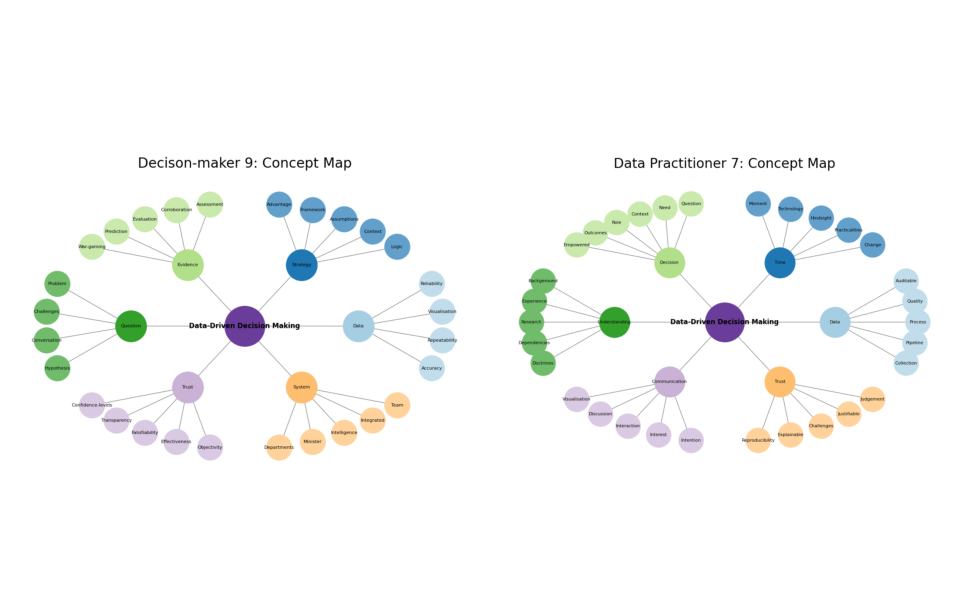
\includegraphics{210431461_CSC8639_Dissertation_files/figure-latex/ConceptMapExample-1.pdf}
\vspace{-3.3cm}

The findings from this user research indicate that decision-makers need
transparency of how the data is used to trust the insights informing
data-driven decisions. This suggests that endeavors to create greater
transparency in data pipelines, such as the research outlined in the
subsequent sections of this paper, are worthy of further study. It also
suggests that evaluating the objectivity and quality of data sources as
well as mechanisms to develop common descriptions of data insight
confidence-levels are potential avenues for data science to have greater
policy impact.

It is important to reiterate that the findings of this user research are
limited; bias is introduced because the small number of participants are
selected from the researcher's professional network. However, given the
consistency of insights from the user research participants, further
interviews with a wider, random subset of the population would be
beneficial.

\hypertarget{analysis-methodology}{%
\section{ANALYSIS METHODOLOGY}\label{analysis-methodology}}

This section outlines the analysis design undertaken to explain the
impact of downsampling algorithms on time series data without detailing
extensive statistical evidence; the decisions, justifications and
limitations of this methodology are shared.

\textbf{4.1 Data}

The eight Alan Turing Institute \texttt{Annotated\ Change}
\protect\hyperlink{ref-ATIChangePoint}{{[}39{]}} synthetic time series
are selected for initial analysis. These time series have been selected
because they are previously cleaned time series from a reputable
institution with known change points that are designed to provide
examples of different types of time series. However, there is an
inherent limitation in using synthetic time series for analysis because
the data has been generated for a different purpose. These synthetic
time series (demo\_100, demo\_200, demo\_300, demo\_400, demo\_500,
demo\_600, demo\_700, demo\_800) are used for demonstration to support
change point annotators annotate real-world data sets for the
\texttt{Turing\ Change\ Point\ Dataset}
\protect\hyperlink{ref-ATIChangePoint}{{[}39{]}}. The eighth
\texttt{Annotated\ Change} synthetic time series (demo\_800) is
multivariate and split in two (800A and 800B) to create nine synthetic
time series for this research and enable better comparison.

\textbf{4.2 Downsampling}

These nine synthetic time series are imported into \texttt{RStudio} from
JSON scripts and two downsampling algorithms are applied to all with
the\texttt{Jettison\ MVP\ Code}
\protect\hyperlink{ref-Jettison}{{[}40{]}}. This enables initial
insights into the impacts of downsampling with minimally complex code.
The two algorithms used by the \texttt{Jettison\ MVP\ Code}
\protect\hyperlink{ref-Jettison}{{[}40{]}} are \emph{EveryNth}, which
selects every other data point, and \emph{Percentage Change}, which
selects every data point that has greater than one per cent difference
between the last transmitted and newest values.

The \texttt{Jettison\ MVP\ Code}
\protect\hyperlink{ref-Jettison}{{[}40{]}} applies these algorithms
iteratively across each of the nine synthetic time series. This creates
parameters 1 to 50 for each downsampling algorithm and
\texttt{Annotated\ Change} time series. There are now 900 time series
for investigation; 450 for each downsampling algorithm.

The R package \texttt{imputeTS}
\protect\hyperlink{ref-imputeTS_R}{{[}15{]}} is applied to all 900 time
series to obtain the remaining data volume after downsampling, number of
missing values (NAs), and number of gaps in the time series. This is
important to understand the effect of each downsampling algorithm.
Initial analysis highlights that the effect of each downsampling
algorithm is unevenly distributed across the 50 parameters; for example,
\emph{EveryNth} discards data more quickly than \emph{Percentage Change}
so comparing the time series for each parameter is insufficient. The
remaining data volume, therefore, provides a common variable that
enables like-for-like comparison between the downsampling algorithms and
their impact.

The missing values for each of the 900 time series are replaced by the
\texttt{imputeTS} linear interpolation function. This is a simple
imputation algorithm that returns each time series to its original
length and is a commonly used approach to present line graphs {[}ADD
REFERENCE{]}. The selection of this simple imputation function may limit
the findings of this analysis, but returning the time series to their
original length enables a like-for-like comparison of downsampling
impact. For each \texttt{Annotated\ Change} synthetic time series there
is now an imputed time series for parameters 1 to 50 and each
downsampling algorithm.

\textbf{4.3 Features}

The \texttt{Rcatch22} package
\protect\hyperlink{ref-catch22_R}{{[}16{]}} enables the computation of a
value for each of the catch22 time series features
\protect\hyperlink{ref-catch22}{{[}34{]}}. Values for the 22 time series
features are calculated for each of the nine original synthetic time
series and 900 imputed time series. The difference between the original
and imputed time series feature values is calculated and that difference
scaled to accurately compare how the downsampling algorithms impact
these catch22 features. The standard deviation across the 900 imputed
time series for each catch22 feature is also calculated to indicate the
sensitivity of each time series feature to downsampling. The catch22
features are considered to be more sensitive if the standard deviation
across the 900 imputed time series is higher.

The application of catch22 features in this way is potentially limited;
the time series features reflect characteristics that help cluster and
classify different time series. Further analysis is needed to confirm
whether features sensitive to downsampling are applicable to all time
series types.

\textbf{4.4 Visualisation}

Combining \texttt{imputeTS} \protect\hyperlink{ref-imputeTS_R}{{[}15{]}}
and \texttt{Rcatch22} \protect\hyperlink{ref-catch22_R}{{[}16{]}} in
this way is unstudied; initial visual analysis to observe the impact of
downsampling on catch22 features is conducted utilising bar and line
graphs alongside heatmaps. All the decision-makers who were interviewed
as part of the aforementioned user research emphaised the importance of
visualisation in data transparency and data-driven decision-making. In
line with this, different approaches to visualising the impact of
downsampling are tried to explore how best the impact of downsampling
could be visually communicated by data practitioners for
decision-makers. However, the visualisations created by this research
are under-developed; usability research needs to be conducted with
decision-makers and data practitioners to ensure the visualisations meet
the aim of this research.

\hypertarget{results-and-evaluation}{%
\section{RESULTS AND EVALUATION}\label{results-and-evaluation}}

\vspace{-0.38cm}

This section shares the results of this research with a discussion of
their the limitations and potential avenues for further investigation;
these results are presented in three themes: downsampling sensitivity,
downsampling impact, and feature variation.

\textbf{5.1 Downsampling sensitivity}

Seven catch22 features appear to show a wider dispersion across the 900
imputed time series than the other 15 features. These seven features are
considered to be more sensitive to the impacts of downsampling. To
demonstrate the sensitivity of these seven features, features with the
highest standard deviation across all the imputed time series are
visualised in the bar graph below. The standard deviation of all 22
features is shared in Annex B.

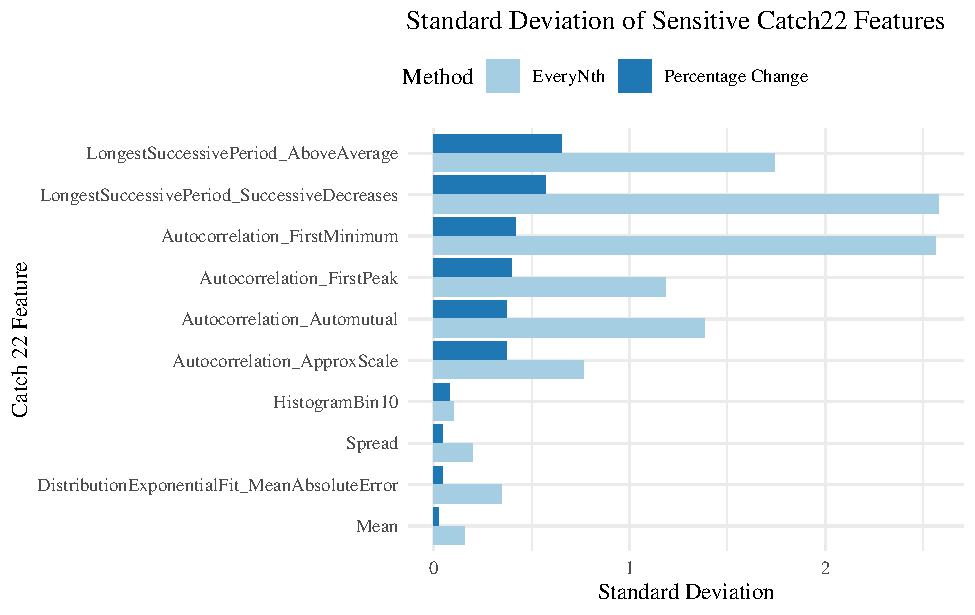
\includegraphics{210431461_CSC8639_Dissertation_files/figure-latex/CombinedSensitivity-1.pdf}

Figure 2 suggests that the \emph{EveryNth} algorithm impacts the catch22
time series features more than the \emph{Percentage Change} algorithm.
Initial analysis indicates that this is because the \emph{EveryNth}
algorithm discards more data, more quickly in the 50 parameters of
downsampling. The sensitivity of these features to the \emph{Percentage
Change} is limited by the number of parameters used for this research.
It would be beneficial to investigate the impact of \emph{Percentage
Change} further by creating downsampling parameters beyond 50 until the
same volume of data is discarded by both algorithms.

The standard deviation of the seven most sensitive catch22 features is
presented in the table below. This table includes the standard deviation
of these features for the \emph{EveryNth} algorithm (`everyNth'), the
\emph{Percentage Change} algorithm (`PercentageChange'), and the
combined standard deviation (`Combined').

\begin{table}[H]

\caption{\label{tab:unnamed-chunk-2}Standard Deviation of the Seven Most Sensitive Catch22 Features}
\centering
\begin{tabular}[t]{l|r|r|r}
\hline
Feature & everyNth & PercentageChange & Combined\\
\hline
Autocorr\_FirstMinimum & 2.5639294 & 0.4181318 & 2.5253400\\
\hline
LongestPeriod\_Decreases & 2.5778227 & 0.5711553 & 2.0901832\\
\hline
LongestPeriod\_AboveAverage & 1.7389139 & 0.6524714 & 1.7545755\\
\hline
Autocorr\_Automutual & 1.3808674 & 0.3736266 & 1.3890246\\
\hline
Autocorr\_FirstPeak & 1.1844657 & 0.3954080 & 0.9515096\\
\hline
Autocorr\_ApproxScale & 0.7661026 & 0.3713025 & 0.7172823\\
\hline
DistributionExponentialFit\_MAE & 0.3440829 & 0.0437543 & 0.3605538\\
\hline
\end{tabular}
\end{table}

\vspace{-0.5cm}

The combined standard deviation is used to identify the seven catch22
features that appear to be most sensitive. Table 2 suggests that the
first minimum of the autocorrelation function (`Autocorr\_FirstMinimum'
or `CO\_FirstMin\_ac') is most sensitive across both of the algorithms;
that the catch22 feature measuring the longest sequence of successive
steps that decrease (`LongestPeriod\_Decrease' or
`SB\_BinaryStats\_diff\_longstretch0') is most sensitive to the
\emph{EveryNth} algorithm; and, the longest sequence of successive
values greater than the mean (`LongestPeriod\_AboveAverage' or
`SB\_BinaryStats\_mean\_longstretch1') is most sensitive to the
\emph{Percentage Change} algorithm.

These results indicate that it may be possible to communicate the impact
of downsampling via the sensitivity of the catch22 features. However,
standard deviation is a limited measure that suggests, rather than
confirms, sensitivity to the impacts of downsampling algorithms. Further
statistical analysis is needed to confirm that the changes in the
features is directly caused by the impact of downsampling.

\textbf{5.2 Downsampling Impact}

Identifying that seven catch22 features appear to be more sensitive to
the impacts of downsampling enables data practitioners to evaluate and
communicate the impact of different downsampling algorithms without deep
statistical analysis. The difference between the values of catch22
features for the nine original time series and 900 imputes time series
is used to measure the impact of downsampling. The heapmap below
visualises this difference, scaled, for the seven most sensitive catch22
features across the 900 imputed time series and each of the 50
parameters.

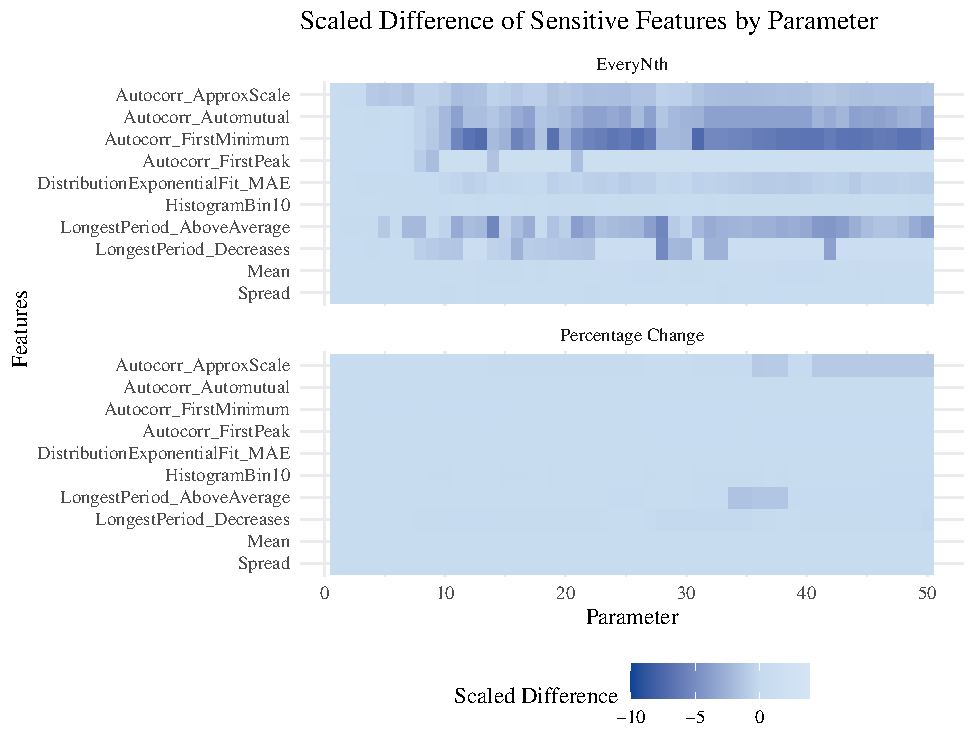
\includegraphics{210431461_CSC8639_Dissertation_files/figure-latex/Heatmap_param-1.pdf}

Figure 3 suggests that the approximate scale of autocorrelation
(`Autocorr\_ApproxScale' or `CO\_f1ecac') and the longest sequence of
successive values greater than the mean (`LongestPeriod\_AboveAverage'
or `SB\_BinaryStats\_mean\_longstretch1') are the first catch22 features
to be impacted by the downsampling algorithms. Interestingly, figure 3
also demonstrates that the catch22 features that are impacted by both
downsampling algorithms tend to increase in comparison the original
feature values; this dynamic warrants further statistical evaluation.

However, the parameters prevent a like-for-like comparison of the two
downsampling algorithms as \emph{EveryNth} discards data more quickly
than \emph{Percentage Change}. The heatmap below also visualises the
scaled difference between the values of the original catch22 features
and the imputed time series, but across the volume of data retained by
the downsampling algorithms before \texttt{imputeTS}
\protect\hyperlink{ref-imputeTS_R}{{[}15{]}} imputed the missing values.

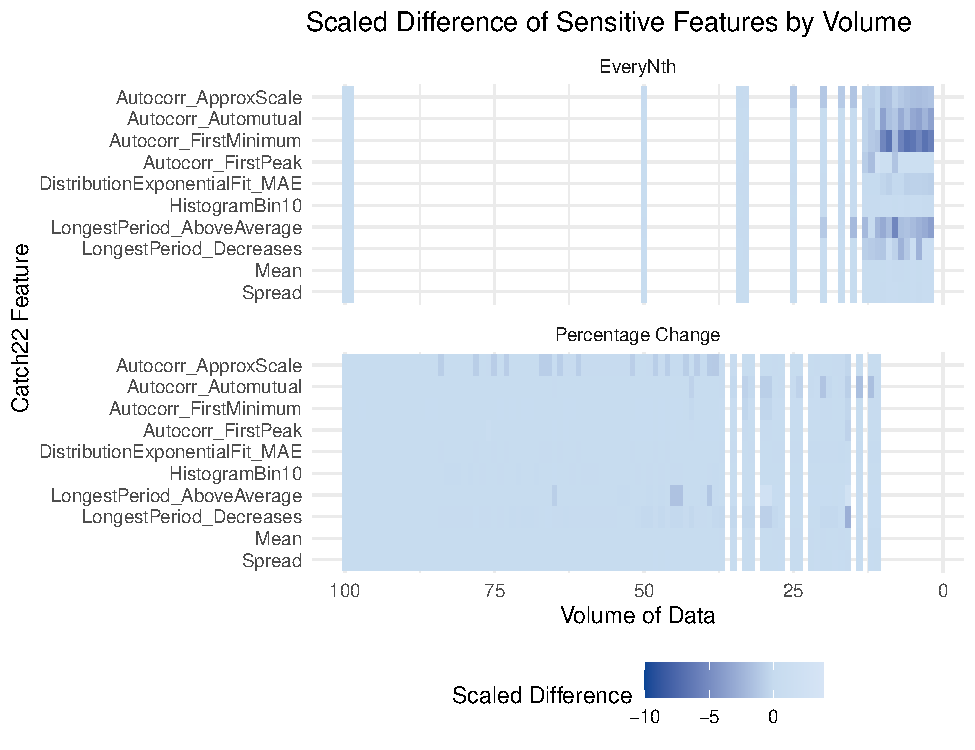
\includegraphics{210431461_CSC8639_Dissertation_files/figure-latex/Heatmap_vol-1.pdf}

Figure 4 demonstrates that data volume retained by the downsampling
algorithms creates acute differences, especially when less than 20 data
points remained after \emph{EveryNth} is applied. Interestingly, the
impact of \emph{Percentage Change} appears to be inconsistent; there are
some retained data volumes where \texttt{Autocorr\_ApproxScale} and
\texttt{LongestPeriod\_AboveAverage} do not appear to be impacted by
\emph{Percentage Change} even though larger retained data volumes appear
to be impacted; this dynamic warrants further investigation.

Downsampling can perturb the the statistical properties {[}ADD
REFERENCE{]} and visual perception {[}ADD REFERENCE{]} of the data.
Catch2 features are statistical properties of time series. It is likely
that some of these statistical properties will be more or less effected
by downsampling because downsampling algorithms preserve different data
points from the original time series. A full table of the statistical
properties represented by each catch22 feature is shared in Annex C.

It is not possible, however, to understand the impact of both
downsampling algorithms from this visualisation. The \emph{Percentage
Change} algorithm needs to be applied for more than 50 parameters so
that it discards volumes of data comparable to the \emph{EveryNth}
algorithm. Despite this, the heatmap visualisation of downsampling
impact holds potential; figure 4 suggests that, with the same volume of
data, the downsampling algorithms impact the catch22 features
differently.

\textbf{5.3 Feature Variation}

The impact of both downsampling algorithms on the most sensitive
features appears to vary across different time series types. This is
exemplified by the catch22 feature `Autocorr\_FirstMinimum'
(`CO\_FirstMin\_ac'): the first minimum of the autocorrelation function
(`Autocorr\_FirstMinimum' or `CO\_FirstMin\_ac.' This feature has the
highest combined standard deviation across the 900 imputed time series
represents \emph{``the number of steps into the future at which a value
of the time series at the current point and that future point remain
substantially (\textgreater1/e) correlated''}
\protect\hyperlink{ref-feature_book}{{[}41{]}}. The line graphs below
highlight how this feature changes over the time series interpolated
from different volumes of data after both downsampling algorithms are
applied. The differences between the catch22 feature value of the
original and imputed time series has been scaled for better comparisons.

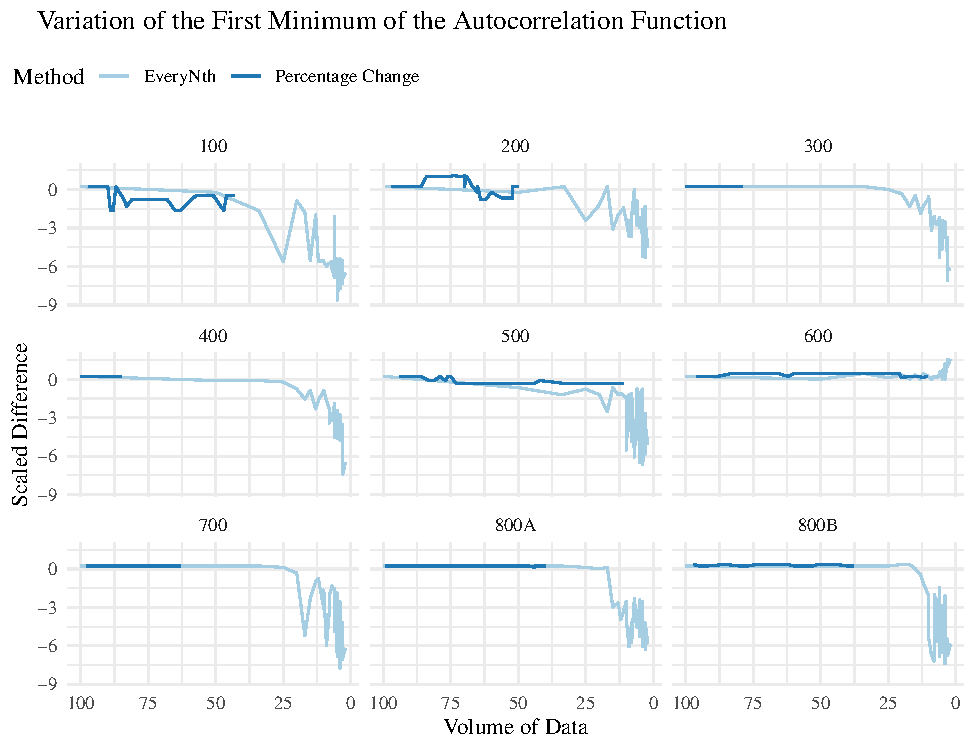
\includegraphics{210431461_CSC8639_Dissertation_files/figure-latex/FirstMinimum-1.pdf}

Figure 5 presents the impact of discarding data for both downsampling
algorithms; the volume of data retained by the \emph{Percentage Change}
algorithm varies by the type of time series whereas the volume of data
retained by the \emph{EveryNth} algorithm trends towards zero. The line
graphs presented in figure 5 highlight how different downsampling
algorithms may more or less preserve the integrity of different time
series. For example, time series `100,' `200' and `600' appear to be
more impacted by the \emph{Percentage Change} algorithm. How the most
sensitive catch22 time series features vary across the different time
series types is shared in Annex D

This variation of downsampling algorithms across time series types
causes the author to question whether the downsampling sensitivity of
catch22 features may vary across time series type too. An example of
this dynamic is visualised by the line graphs below in figure 6, which
plot the scaled difference of the six most sensitive catch22 features
for time series `500.' Time series `500' was selected as more data is
discarded by the \emph{Percentage Change} algorithm, offering a better
comparison.

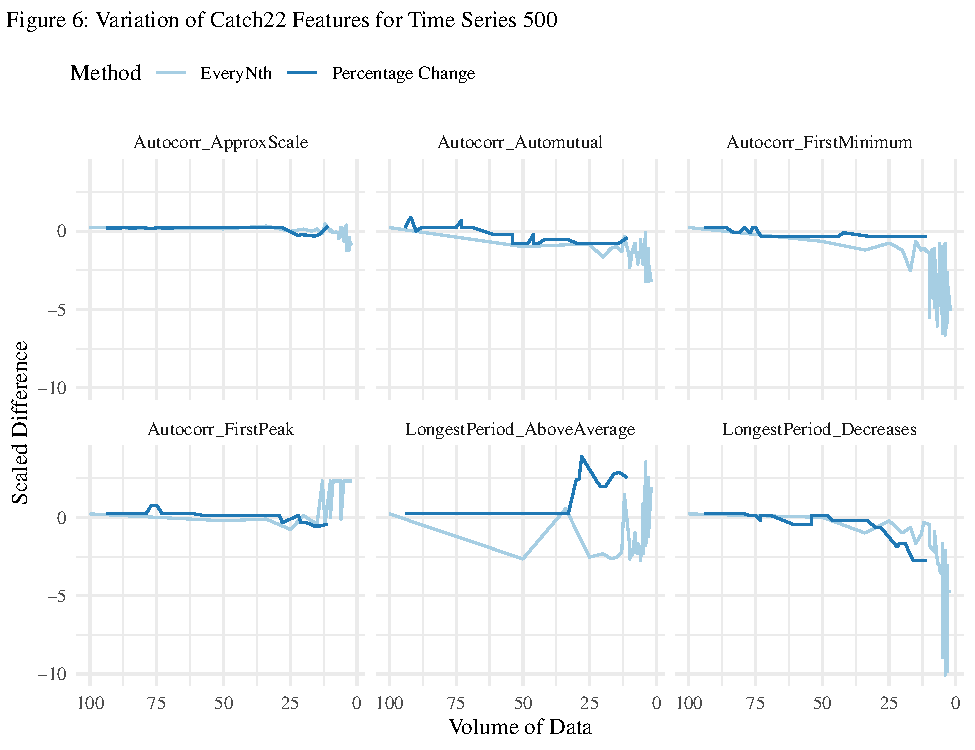
\includegraphics{210431461_CSC8639_Dissertation_files/figure-latex/Catch22Variation-1.pdf}

Figure 6 highlights that, although `Autocorr\_FirstMinimum' is
identified as the most sensitive across both downsampling algorithms,
`Autocorr\_Automutual' might better indicate the impact for time series
`500.' `Autocorr\_Automutual' is the minimum of the automutual
information function (`Autocorr\_Automutual' or
`IN\_AutoMutualInfoStats\_40\_gaussian\_fmmi'); this catch22 feature
outputs a measure of ``autocorrelation in the time series, as the
minimum of the automutual information function''
\protect\hyperlink{ref-feature_book}{{[}41{]}}.

A comparison of the most senstive features for each time series type is
shared in Annex E. It would be beneficial to explore this further as
this variation may offer data practitioners a method for identifying
subsets of features that best indicate the preservation of different
time series.

\hypertarget{future-work}{%
\section{FUTURE WORK}\label{future-work}}

There are many avenues for future work to better understand the
findings, and address the limitations, of this research.

\textbf{6.1 User research}

Additional analysis on the transcripts and recordings of the user
research would be beneficial. For example, using other natural language
processing techniques, such as topic modelling, to better identify the
connections between the key themes identified. It would also be helpful
to conduct user research with a wider group of decision-makers and data
practitioner to develop statistically significant findings for the UK
Government.

Usability research with decision-makers and data practitioners would
also beneficial. Usability would contribute to the refinement of
visualisations so that they better communicate the impact of
downsampling on different time series. How these visualisations perturb
the decision-makers' and data practitioners' perception of downsampling
impact is an important avenue of further investigation.

\textbf{6.2 Downsampling Sensitivity}

It would be beneficial to use the data pipeline developed by C. H. Lubba
et. al \protect\hyperlink{ref-catch22}{{[}34{]}} to generate other
subsets of time series features for distinct tasks in different domains.
Examining the downsampling sensitivity of new subsets of catch22
features is likely to generate the information needed to understand why
certain features are more sensitive to downsampling across different
types of time series.

\textbf{6.3 Downsampling Impact}

Further iterations of dowsampling on the synthetic time series used in
this research is an important to address the limitation of this
research. These iterations will enable a better comparison of the
\emph{EveryNth} and \emph{Percentage Change} algorithms. Equally,
repeating the analysis methodology of this research for other
downsampling algorithms, such as LTTB, as well as applying utilising the
real-world time series shared by the Alan Turing Change Point Data set
will allow a more indept investigation into the impact of downsampling.

These avenues of future work are also vital for generating the
information needed to fully realise the ambitions of this research -
developing comparative visualisations to better communicate the impact
of downsampling on time series. These visualisations should also be
evaluated with users through usability research.

\textbf{6.4 Feature Variation}

Combined, the future work to better understand downsampling impact and
sensitivity could enable the development of thresholds and benchmarks
for downsampling impact variation across time series features and types.
This avenue of further investiation could enable the most relevant and
sensitive time series features to be embedded for proactive downsampling
that reduces the demand on computing resources. For example, embedding
the most sensitive features in smart sensors monitoring a particular
type of time series would enable downsampling at the point of
collection, reducing demand on computing resources for storage. Such
tailoring of downsampling could also facilitate more nuanced discussions
between decision-makers and data practitioners on the thresholds of
downsampling for different decision types to ensure that insights from
downsampled data are used within the bounds of their limitations.

\hypertarget{conclusion}{%
\section{CONCLUSION}\label{conclusion}}

Increasing volumes of time series data are being widely generated and
used by industry and research \protect\hyperlink{ref-TVStore}{{[}10{]}};
downsampling is a vital data processing technique for reducing this
volume, addressing limitations like processing time, computing costs,
storage capabilities, and sustainability ambitions
\protect\hyperlink{ref-TVStore}{{[}10{]}}--\protect\hyperlink{ref-Shift}{{[}12{]}}.
However, downsampling can perturb the statistical properties and visual
perception of time series, potentially impacting the insights that
inform data-driven decisions.

Interviews with 16 UK Civil Servants (nine decision-makers and seven
data practitioners) highlight the importance of transparency in enabling
data-driven decision-making across government. Decision-makers shared
that there is a spectrum of transparency, which depends on the question
being addressed by the data; it's complexity, importance and potential
impact. To trust the data informing data-driven decisions,
decision-makers and data practitioners repeatedly requested transparency
of the data context, source and limitations as well as an assessment of
overall confidence in the data. This user research indicates that
decision-makers need transparency of how the data is used to trust the
insights informing data-driven decisions.

There are seven catch22 time series features
\protect\hyperlink{ref-catch22}{{[}34{]}} that appear to be more
sensitive to the impacts of downsampling. Catch2 features are
statistical properties of time series so they are more or less effected
by downsampling depending on which data points are preserved from the
original time series. The impact of the \emph{everyNth} and
\emph{Percentage Change} downsampling algorithms on the most sensitive
features appears to vary across different time series types. The
downsampling sensitivity of catch22 features also appear to vary across
time series. These results suggest that different subsets of catch22
features could be selected to best indicate the preservation of time
series after downsampling.

The varying sensitivity of catch22 features to different downsampling
algorithms is previously unstudied; this research offers a new
visualisation methodology for data practitioners to communicate the
impact of downsampling on different decisions and create meaningful
transparency about the downsampling choices they are making throughout
the data processing pipeline. This could help decision-makers to trust
the data informing their decisions, supporting decision-makers to
understand the limitations of the data available and the thresholds at
which the data insights can or cannot be relied upon for each decision.

\hypertarget{references}{%
\section*{REFERENCES}\label{references}}
\addcontentsline{toc}{section}{REFERENCES}

\hypertarget{refs}{}
\begin{CSLReferences}{0}{0}
\leavevmode\vadjust pre{\hypertarget{ref-data2017}{}}%
\CSLLeftMargin{{[}1{]} }
\CSLRightInline{Cabinet Office and Government Digital Service,
{``Government transformation strategy: Better use of data.''} HM
Government;
\url{https://www.gov.uk/government/publications/government-transformation-strategy-2017-to-2020/government-transformation-strategy-better-use-of-data},
2017.}

\leavevmode\vadjust pre{\hypertarget{ref-data2020}{}}%
\CSLLeftMargin{{[}2{]} }
\CSLRightInline{Department for Digital, Culture, Media \& Sport and
Department for Science, Innovation \& Technology, {``National data
strategy.''} HM Government;
\url{https://www.gov.uk/government/publications/uk-national-data-strategy/national-data-strategy},
2020.}

\leavevmode\vadjust pre{\hypertarget{ref-data2021}{}}%
\CSLLeftMargin{{[}3{]} }
\CSLRightInline{M. of Defence, {``Data strategy for defence,''}
\emph{GOV.UK}. HM Government;
\url{https://www.gov.uk/government/publications/data-strategy-for-defence/data-strategy-for-defence},
2021.}

\leavevmode\vadjust pre{\hypertarget{ref-data2022}{}}%
\CSLLeftMargin{{[}4{]} }
\CSLRightInline{Central Digital \& Data Office, {``Transforming for a
digital future: 2022 to 2025 roadmap for digital and data.''} HM
Government;
\url{https://www.gov.uk/government/publications/roadmap-for-digital-and-data-2022-to-2025/transforming-for-a-digital-future-2022-to-2025-roadmap-for-digital-and-data},
2022.}

\leavevmode\vadjust pre{\hypertarget{ref-trust}{}}%
\CSLLeftMargin{{[}5{]} }
\CSLRightInline{Centre for Data Ethics \& Innovation, {``Addressing
trust in public sector data use.''}
\url{https://www.gov.uk/government/publications/cdei-publishes-its-first-report-on-public-sector-data-sharing/addressing-trust-in-public-sector-data-use\#introduction--context}.}

\leavevmode\vadjust pre{\hypertarget{ref-datapoint}{}}%
\CSLLeftMargin{{[}6{]} }
\CSLRightInline{J. Donckt, J. Donckt, M. Rademaker, and S. Hoecke,
{``Data point selection for line chart visualization: Methodological
assessment and evidence-based guidelines.''} 2023. doi:
\href{https://doi.org/10.48550/arXiv.2304.00900}{10.48550/arXiv.2304.00900}.}

\leavevmode\vadjust pre{\hypertarget{ref-MinMaxLTTB}{}}%
\CSLLeftMargin{{[}7{]} }
\CSLRightInline{J. Donckt, J. Donckt, M. Rademaker, and S. Hoecke,
{``MinMaxLTTB: Leveraging MinMax-preselection to scale LTTB.''}
\url{https://arxiv.org/abs/2305.00332}, 2023.}

\leavevmode\vadjust pre{\hypertarget{ref-pathway}{}}%
\CSLLeftMargin{{[}8{]} }
\CSLRightInline{Government Analysis Function, {``Types of data in
government learning pathway.''}
\url{https://analysisfunction.civilservice.gov.uk/learning-development/learning-pathways/types-of-data-in-government-learning-pathway/},
2022.}

\leavevmode\vadjust pre{\hypertarget{ref-onstool}{}}%
\CSLLeftMargin{{[}9{]} }
\CSLRightInline{Office for National Statistics, {``Time series
explorer.''}
\url{https://www.ons.gov.uk/timeseriestool?query=\&topic=\&updated=\&fromDateDay=\&fromDateMonth=\&fromDateYear=\&toDateDay=\&toDateMonth=\&toDateYear=\&size=50},
Unknown.}

\leavevmode\vadjust pre{\hypertarget{ref-TVStore}{}}%
\CSLLeftMargin{{[}10{]} }
\CSLRightInline{Y. An, Y. Su, Y. Zhu, and J. Wang, {``TVStore:
Automatically bounding time series storage via time-varying
compression,''} in \emph{Proceedings of the 20th USENIX conference on
file and storage technologies}, in USENIX conference on file and STorage
technologies. Santa Clara, CA, USA: USENIX Association, 2022, pp.
83--99.}

\leavevmode\vadjust pre{\hypertarget{ref-Sveinn}{}}%
\CSLLeftMargin{{[}11{]} }
\CSLRightInline{S. Steinarsson, {``Downsampling time series for visual
representation.''} University of Iceland, Faculty of Industrial
Engineering, Mechanical Engineering; Computer Science, School of
Engineering; Natural Sciences, University of Iceland, Reykjavik,
Iceland, 2013.}

\leavevmode\vadjust pre{\hypertarget{ref-Shift}{}}%
\CSLLeftMargin{{[}12{]} }
\CSLRightInline{The Shift Project, {``Implementing digital
sufficiency,''} 2020.}

\leavevmode\vadjust pre{\hypertarget{ref-downsampling}{}}%
\CSLLeftMargin{{[}13{]} }
\CSLRightInline{W. Aigner, S. Miksch, W. Muller, H. Schumann, and C.
Tominski, {``Visual methods for analyzing time-oriented data,''}
\emph{IEEE Transactions on Visualization and Computer Graphics}, vol.
14, no. 1, pp. 47--60, 2008, doi:
\href{https://doi.org/10.1109/TVCG.2007.70415}{10.1109/TVCG.2007.70415}.}

\leavevmode\vadjust pre{\hypertarget{ref-sampling}{}}%
\CSLLeftMargin{{[}14{]} }
\CSLRightInline{B. C. Kwon, J. Verma, P. J. Haas, and C. Demiralp,
{``Sampling for scalable visual analytics,''} \emph{IEEE Computer
Graphics and Applications}, vol. 37, no. 1, pp. 100--108, 2017, doi:
\href{https://doi.org/10.1109/MCG.2017.6}{10.1109/MCG.2017.6}.}

\leavevmode\vadjust pre{\hypertarget{ref-imputeTS_R}{}}%
\CSLLeftMargin{{[}15{]} }
\CSLRightInline{S. Moritz and T. Bartiz-Beielstein, {``imputeTS: Time
series missing value imputation in r,''} vol. 9.1.
\url{https://github.com/SteffenMoritz/imputeTS}; R Journal, 2017. doi:
\href{https://doi.org/10.32614/RJ-2017-009}{10.32614/RJ-2017-009}.}

\leavevmode\vadjust pre{\hypertarget{ref-catch22_R}{}}%
\CSLLeftMargin{{[}16{]} }
\CSLRightInline{C. H. Lubba, B. Fulcher, T. Henderspn, B. Harris, O. r.
TL, and O. Cliff, {``catch22: CAnonical time-series CHaracteristics.''}
\url{https://github.com/DynamicsAndNeuralSystems/catch22}; R Journal,
2022. doi:
\href{https://doi.org/10.5281/zenodo.6673597}{10.5281/zenodo.6673597}.}

\leavevmode\vadjust pre{\hypertarget{ref-political_transparency}{}}%
\CSLLeftMargin{{[}17{]} }
\CSLRightInline{K. E. Levy and D. M. Johns, {``When open data is a
trojan horse: The weaponization of transparency in science and
governance,''} \emph{Big Data \& Society}, vol. 3, no. 1, 2016, doi:
\href{https://doi.org/10.1177/2053951715621568}{10.1177/2053951715621568}.}

\leavevmode\vadjust pre{\hypertarget{ref-social_transparency}{}}%
\CSLLeftMargin{{[}18{]} }
\CSLRightInline{J. Bates, H. Kennedy, I. Medina Perea, S. Oman, and L.
Pinney, {``Socially meaningful transparency in data-based systems:
Reflections and proposals from practice,''} \emph{Journal of
Documentation}, vol. ahead--of--print, 2023, doi:
\href{https://doi.org/10.1108/JD-01-2023-0006}{10.1108/JD-01-2023-0006}.}

\leavevmode\vadjust pre{\hypertarget{ref-transparency_lack}{}}%
\CSLLeftMargin{{[}19{]} }
\CSLRightInline{M. Ananny and K. Crawford, {``Seeing without knowing:
Limitations of the transparency ideal and its application to algorithmic
accountability,''} \emph{New Media \& Society}, vol. 20, no. 3, pp.
973--989, 2018, doi:
\href{https://doi.org/10.1177/1461444816676645}{10.1177/1461444816676645}.}

\leavevmode\vadjust pre{\hypertarget{ref-digital_transparency}{}}%
\CSLLeftMargin{{[}20{]} }
\CSLRightInline{R. Matheus, M. Janssen, and T. Janowski, {``Design
principles for creating digital transparency in government,''}
\emph{Government Information Quarterly}, vol. 38, no. 1, 2021, doi:
\href{https://doi.org/10.1016/j.giq.2020.101550}{10.1016/j.giq.2020.101550}.}

\leavevmode\vadjust pre{\hypertarget{ref-transparency_obfuscation}{}}%
\CSLLeftMargin{{[}21{]} }
\CSLRightInline{N. A. Draper and J. Turow, {``The corporate cultivation
of digital resignation,''} \emph{New Media \& Society}, vol. 21, no. 8,
pp. 1824--1839, 2019, doi:
\href{https://doi.org/10.1177/1461444819833331}{10.1177/1461444819833331}.}

\leavevmode\vadjust pre{\hypertarget{ref-transparency_fallacy}{}}%
\CSLLeftMargin{{[}22{]} }
\CSLRightInline{J. A. Obar, {``Sunlight alone is not a disinfectant:
Consent and the futility of opening big data black boxes (without
assistance),''} \emph{Big Data \& Society}, vol. 7, no. 1, 2020, doi:
\href{https://doi.org/10.1177/2053951720935615}{10.1177/2053951720935615}.}

\leavevmode\vadjust pre{\hypertarget{ref-timenotes}{}}%
\CSLLeftMargin{{[}23{]} }
\CSLRightInline{J. Walker, R. Borgo, and MW. Jones, {``TimeNotes: A
study on effective chart visualization and interaction techniques for
time-series data,''} \emph{IEEE Transactions on Visualization and
Computer Graphics}, vol. 22, 2016, doi:
\href{https://doi.org/10.1109/TVCG.2015.2467751}{10.1109/TVCG.2015.2467751}.}

\leavevmode\vadjust pre{\hypertarget{ref-plotly}{}}%
\CSLLeftMargin{{[}24{]} }
\CSLRightInline{J. Donckt, J. Donckt, E. Deprost, and S. Hoecke,
{``Plotly-resampler: Effective visual analytics for large time
series,''} \emph{IEEE Visualization and Visual Analytics}, 2022, doi:
\href{https://doi.org/10.1109/VIS54862.2022.00013}{10.1109/VIS54862.2022.00013}.}

\leavevmode\vadjust pre{\hypertarget{ref-imputeTS}{}}%
\CSLLeftMargin{{[}25{]} }
\CSLRightInline{S. Moritz and T. Bartiz-Beielstein, {``imputeTS: Time
series missing value imputation in r.''}
\url{https://cran.r-project.org/web/packages/imputeTS/vignettes/imputeTS-Time-Series-Missing-Value-Imputation-in-R.pdf};
R Journal, 2017.}

\leavevmode\vadjust pre{\hypertarget{ref-storage}{}}%
\CSLLeftMargin{{[}26{]} }
\CSLRightInline{A. Visheratin \emph{et al.}, {``Peregreen {\textendash}
modular database for efficient storage of historical time series in
cloud environments,''} in \emph{2020 USENIX annual technical conference
(USENIX ATC 20)},
\url{https://www.usenix.org/conference/atc20/presentation/visheratin};
USENIX Association, 2020, pp. 589--601.}

\leavevmode\vadjust pre{\hypertarget{ref-CatchUp}{}}%
\CSLLeftMargin{{[}27{]} }
\CSLRightInline{T. Schlossnagle, J. Sheehy, and C. McCubbin,
{``Always-on time-series database: Keeping up where there's no way to
catch up,''} \emph{Commun. ACM}, vol. 64, no. 7, pp. 50--56, 2021.}

\leavevmode\vadjust pre{\hypertarget{ref-IR}{}}%
\CSLLeftMargin{{[}28{]} }
\CSLRightInline{HM Government, {``Global britain in a competitive age:
The integrated review of security, defence, development and foreign
policy.''}
\url{https://www.gov.uk/government/publications/global-britain-in-a-competitive-age-the-integrated-review-of-security-defence-development-and-foreign-policy};
GOV.UK, 2021.}

\leavevmode\vadjust pre{\hypertarget{ref-climate}{}}%
\CSLLeftMargin{{[}29{]} }
\CSLRightInline{I. Foster \emph{et al.}, {``Computing just what you
need: Online data analysis and reduction at extreme scales,''} in
\emph{Euro-par 2017}, F. F. Rivera, T. F. Pena, and J. C. Cabaleiro,
Eds., in Lecture notes in computer science (including subseries lecture
notes in artificial intelligence and lecture notes in bioinformatics).
Germany: Springer Verlag, 2017, pp. 3--19. doi:
\href{https://doi.org/10.1007/978-3-319-64203-1_1}{10.1007/978-3-319-64203-1\_1}.}

\leavevmode\vadjust pre{\hypertarget{ref-dashql}{}}%
\CSLLeftMargin{{[}30{]} }
\CSLRightInline{A. Kohn, D. Moritz, and T. Neumann, {``DashQL --
complete analysis workflows with SQL.''} 2023. doi:
\href{https://doi.org/10.48550/arXiv.2306.03714}{10.48550/arXiv.2306.03714}.}

\leavevmode\vadjust pre{\hypertarget{ref-EveryNth}{}}%
\CSLLeftMargin{{[}31{]} }
\CSLRightInline{U. Jugel, Z. Jerzak, G. Hackenbroic, and V. Markl,
{``VDDA: Automatic visualization-driven data aggregation in relational
databases,''} \emph{The VLDB Journal}, vol. 25, 2016, doi:
\href{https://doi.org/10.1007/s00778-015-0396-z}{10.1007/s00778-015-0396-z}.}

\leavevmode\vadjust pre{\hypertarget{ref-MinMaxOrdered}{}}%
\CSLLeftMargin{{[}32{]} }
\CSLRightInline{W. Yunhai \emph{et al.}, {``OM3: An ordered multi-level
min-max representation for interactive progressive visualization of time
series,''} in \emph{Proc. ACM manag. data}, ACM, 2023. doi:
\href{https://doi.org/10.1145/3589290}{10.1145/3589290}.}

\leavevmode\vadjust pre{\hypertarget{ref-M4}{}}%
\CSLLeftMargin{{[}33{]} }
\CSLRightInline{U. Jugel, Z. Jerzak, G. Hackenbroich, and V. Markl,
{``M4: A visualization-oriented time series data aggregation.
Proceedings of the VLDB endowment,''} vol. 7, 2014.}

\leavevmode\vadjust pre{\hypertarget{ref-catch22}{}}%
\CSLLeftMargin{{[}34{]} }
\CSLRightInline{C. H. Lubba, S. S. Sarab, P. Knaute, S. R. Schultz, B.
D. Fulcher, and N. S. Jones, {``catch22: CAnonical time-series
CHaracteristics,''} \emph{Data Mining and Knowledge Discovery}, vol. 33,
2019, doi:
\href{https://doi.org/10.1007/s10618-019-00647-x}{10.1007/s10618-019-00647-x}.}

\leavevmode\vadjust pre{\hypertarget{ref-fulcher2017}{}}%
\CSLLeftMargin{{[}35{]} }
\CSLRightInline{B. D. Fulcher and N. S. Jones, {``Highly comparative
feature-based time-series classification,''} \emph{IEEE Transactions on
Knowledge and Data Engineering}, vol. 26, no. 12, pp. 3026--3037, 2014,
doi:
\href{https://doi.org/10.1109/TKDE.2014.2316504}{10.1109/TKDE.2014.2316504}.}

\leavevmode\vadjust pre{\hypertarget{ref-bagnall}{}}%
\CSLLeftMargin{{[}36{]} }
\CSLRightInline{A. Bagnall, J. Lines, A. Bostrom, J. Large, and E.
Keogh, {``The great time series classification bake off: A review and
experimental evaluation of recent algorithmic advances,''} \emph{Data
Mining and Knowledge Discovery}, vol. 31, 2017, doi:
\href{https://doi.org/10.1007/s10618-016-0483-9}{10.1007/s10618-016-0483-9}.}

\leavevmode\vadjust pre{\hypertarget{ref-henderson}{}}%
\CSLLeftMargin{{[}37{]} }
\CSLRightInline{T. Henderson and B. D. Fulcher, {``An empirical
evaluation of time-series feature sets,''} in \emph{2021 international
conference on data mining workshops (ICDMW)}, 2021, pp. 1032--1038. doi:
\href{https://doi.org/10.1109/ICDMW53433.2021.00134}{10.1109/ICDMW53433.2021.00134}.}

\leavevmode\vadjust pre{\hypertarget{ref-futzing}{}}%
\CSLLeftMargin{{[}38{]} }
\CSLRightInline{S. Alspaugh, N. Zokaei, A. Liu, C. Jin, and M. A.
Hearst, {``Futzing and moseying: Interviews with professional data
analysts on exploration practices,''} \emph{IEEE Transactions on
Visualization and Computer Graphics}, vol. 25, no. 1, pp. 22--31, 2019,
doi:
\href{https://doi.org/10.1109/TVCG.2018.2865040}{10.1109/TVCG.2018.2865040}.}

\leavevmode\vadjust pre{\hypertarget{ref-ATIChangePoint}{}}%
\CSLLeftMargin{{[}39{]} }
\CSLRightInline{G. J. J. van den Burg and C. K. I. Williams, {``An
evaluation of change point detection algorithms.''}
\url{https://github.com/alan-turing-institute/AnnotateChange}, 2022.
doi:
\href{https://doi.org/10.48550/arXiv.2003.06222}{10.48550/arXiv.2003.06222}.}

\leavevmode\vadjust pre{\hypertarget{ref-Jettison}{}}%
\CSLLeftMargin{{[}40{]} }
\CSLRightInline{M. Forshaw, {``Jettison MVP code.''}
\url{https://github.com/MattForshaw/Jettison/tree/main/MVPCode}, 2023.}

\leavevmode\vadjust pre{\hypertarget{ref-feature_book}{}}%
\CSLLeftMargin{{[}41{]} }
\CSLRightInline{C. H. Lubba, B. Fulcher, T. Henderspn, B. Harris, O. r.
TL, and O. Cliff, {``catch22 features.''}
\url{https://feature-based-time-series-analys.gitbook.io/catch22-features/},
2023.}

\end{CSLReferences}

\bibliographystyle{unsrt}
\bibliography{references.bib}


\end{document}
